%
% teil2.tex -- Beispiel-File für teil2 
%
% (c) 2020 Prof Dr Andreas Müller, Hochschule Rapperswil
%
% !TEX root = ../../buch.tex
% !TEX encoding = UTF-8
%
\section{Richardsons Ansatz \label{geostrophisch:section:richardsonAnsatz}}
\kopfrechts{Richardsons Ansatz}

Richardson wählte einen innovativen, aber im Grunde sehr einfachen Ansatz:  
Statt vereinfachter Modelle verwendete er ein vollständiges System bestehend aus vier Differentialgleichungen.
Die erste Gleichung:
\begin{equation}
	\frac{D\vec{v}}{Dt} + 2\vec{\Omega} \times \vec{v} = -\frac{1}{\rho}\nabla p + \vec{g} \\,
	\label{eq:navstok}
\end{equation}
ist eine Form der Navier-Stokes-Gleichung für rotierende Bezugssysteme.
$\frac{D\vec{v}}{Dt}$ entspricht der zeitlichen Ableitung aller Geschwindigkeitskomponenten in Nord-, Ost- und Vertikalrichtungen. 
Sie beschreibt die Beschleunigung von Luftmassen und ausserdem werden darin die Corioliskraft und der Druckgradient berücksichtigt.

Als nächstes verwendete er die Kontinuitätsgleichung:
\begin{equation}
	\frac{\partial \rho}{\partial t} + \nabla \cdot (\rho \vec{v}) = 0 \\,
	\label{eq:kont}
\end{equation}
welche die Massenerhaltung beschreibt.
Also in anderen Worten die Luft kann nicht verschwinden oder aus dem nichts auftauchen. 

Zudem brauchte er noch eine Gleichung, welche die Energie beschreibt, dazu diente 
\begin{equation}
	\frac{Ds}{Dt} = Q \\.
	\label{eq:enrgy}
\end{equation}
Damit werden Temperaturänderungen durch Transport sowie Expansion und Kompression der Luftmassen ausgedrückt.

Als letztes verwendete er noch das ideale Gasgesetz:
\begin{equation}
	p = \rho R T,
	\label{eq:gasgesetz}
\end{equation}
dieses ist die physikalische Verbindung von Druck, Temperatur und Dichte eines Gases.  

Er konstruierte eine schachbrettartiges Gitter und legte es über die Karte von Europa (Abbildung~\ref{bild:karteEuropa}).
Nun wollte er für jeden dieser Gitterpunkte das beschriebene Gleichungssystem numerisch von Hand lösen.
Alleine dauerten diese Berechnungen sehr lange und somit brauchte er für die Vorhersage viel zu viel Zeit.
Aufgrund dessen hatte Richardson eine Traumvorstellung von einer Einrichtung zur Berechnung der Wettervorhersagen für die ganze Welt.
Diese besteht aus einer grossen Kuppel, welche im Innern eine Weltkarte an der Wand hat. 
Darin sitzen rundherum etwa 64000 Leute, die je zu ihrem zugewiesenen Bereich die Daten der Atmosphäre erhalten und damit die Berechnungen machen müssen. 
Ihre Resultate geben sie an die benachbarten Mitarbeiter weiter und das grosse Rechnen beginnt von vorn. 
In der Mitte auf dem Podest steht eine Art \glqq Dirigent\grqq, welcher den Leuten, die zu langsam oder zu schnell arbeiten, mittels Lampe Signale gibt und diese darauf hinweisen.
Siehe Abbildung~\ref{bild:richardsonsTraum}, eine Illustration von Richardsons Traumvorstellung.  

\begin{figure}
	\centering
	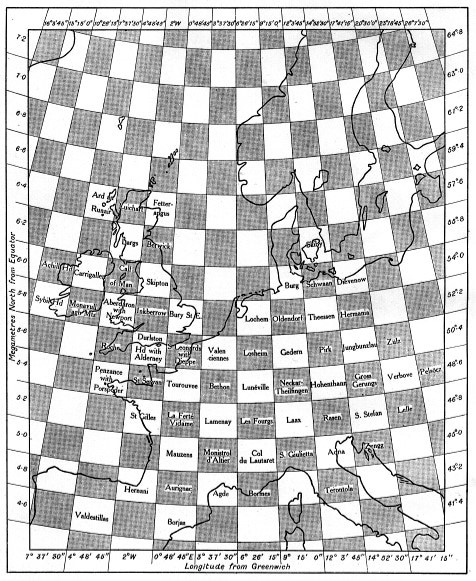
\includegraphics{eingeteilte_Karte.jpg}
	\caption{Gitter zur numerischen Approximation der Felder, welche das Wetter beeinflussen.
		Wie man sehen kann ist das Gitter sehr grob und somit ungenau.
		In der Schweiz zum Beispiel hatt es nur ein Gitterpunkt. 
		}
	\label{bild:karteEuropa}
\end{figure}

\begin{figure}
	\centering
	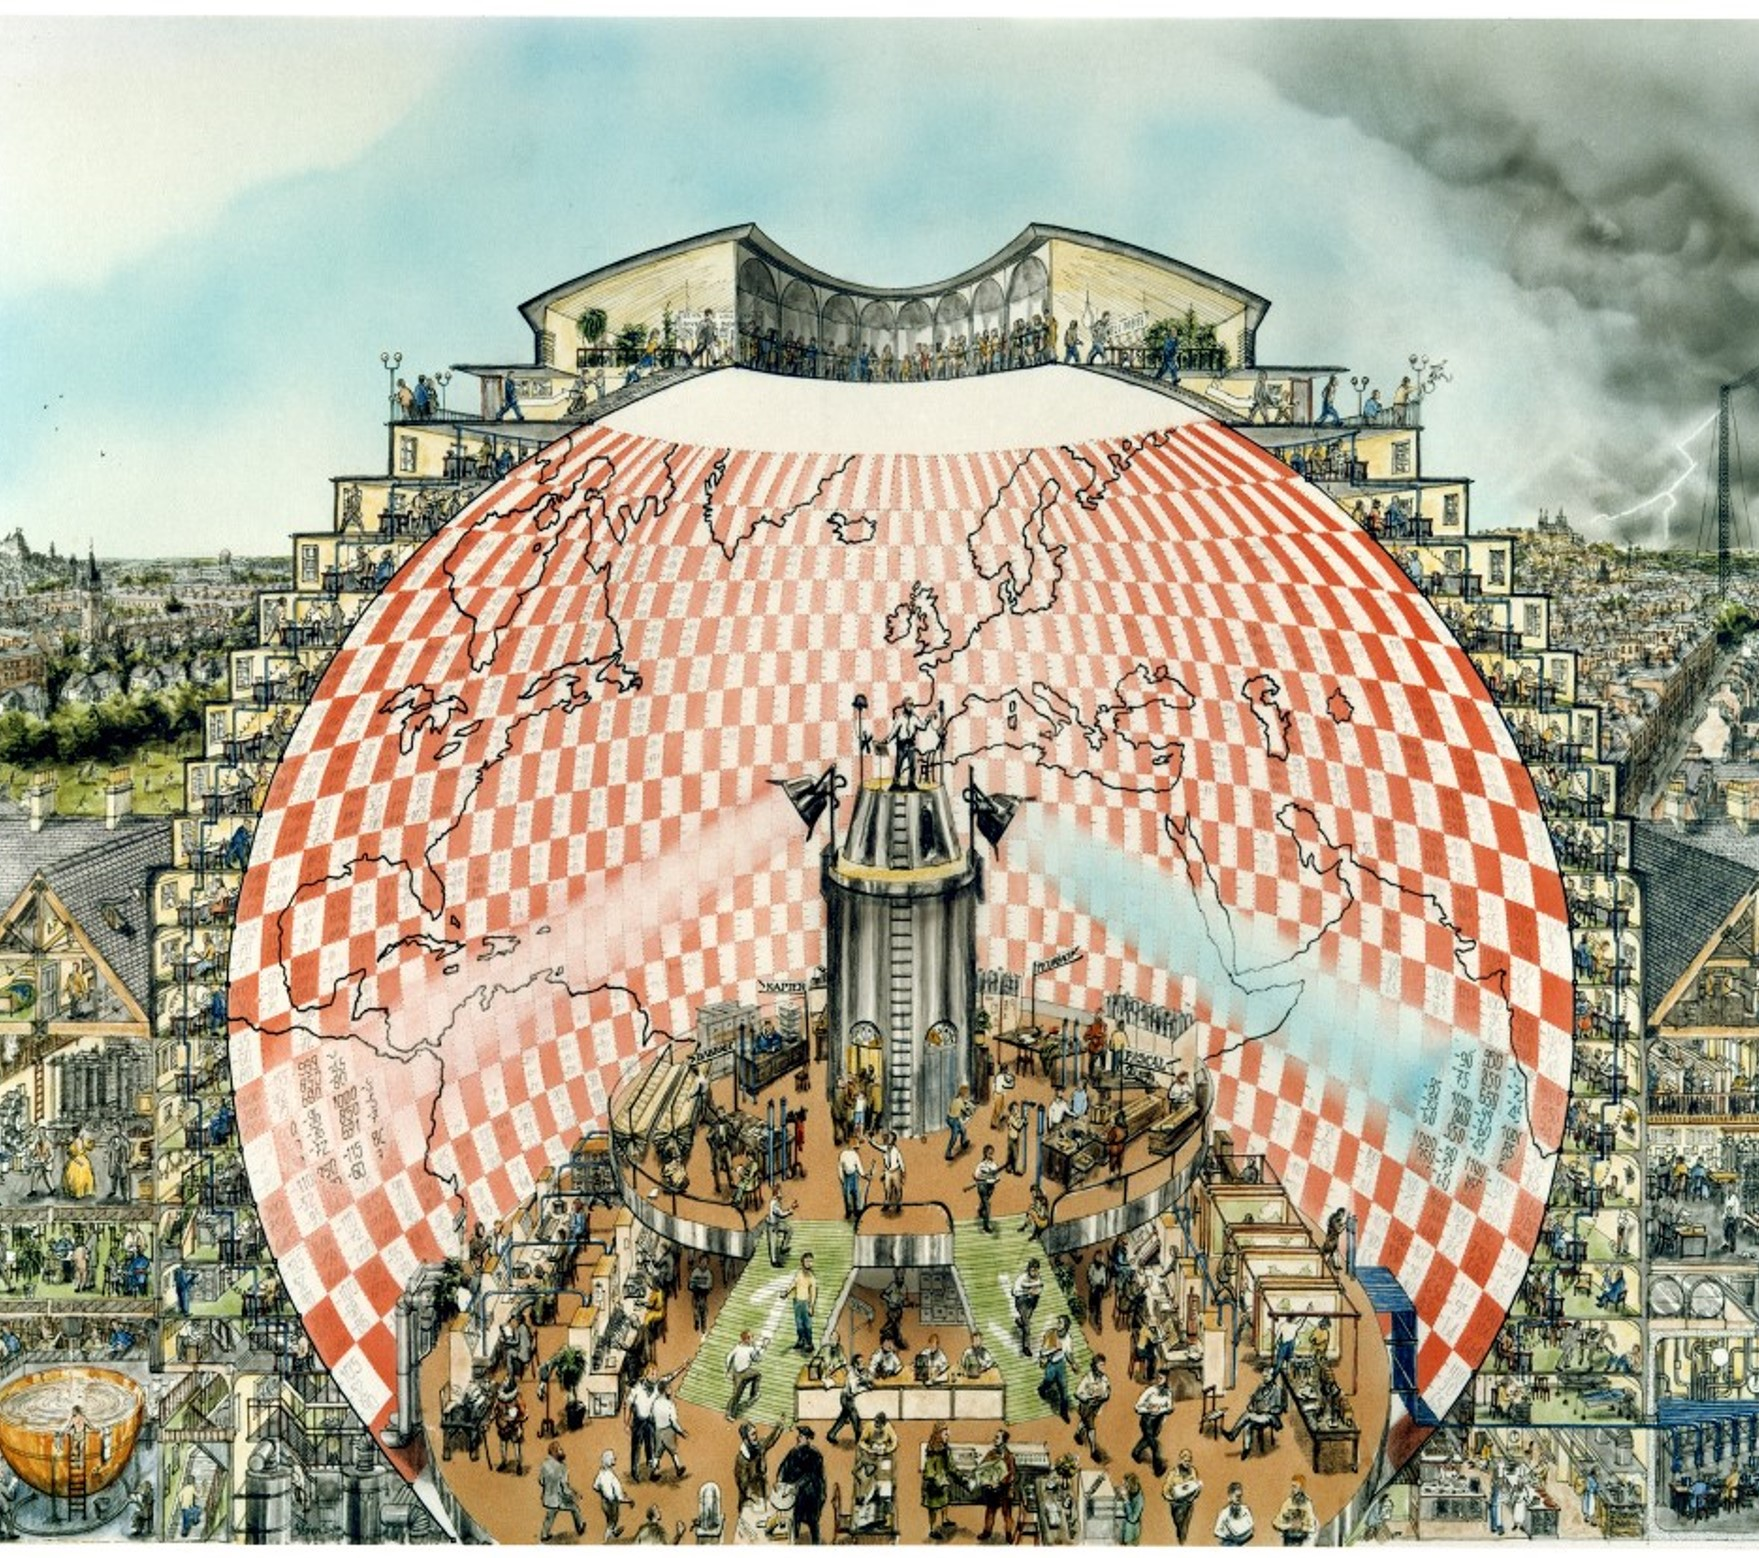
\includegraphics[scale=0.8]{Richardsons_Traum.jpg}
	\caption{Traumvorstellung von Richardson einer Station zur Wettervorhersage. 
	Rundherum hängt eine Weltkarte und Leute berechnen ständig die Atmosphäre zu ihrem Bereich.}
	\label{bild:richardsonsTraum}
\end{figure}

\subsection{Grund der fehlerhaften Vorhersage \label{geostrophisch:subsection:failedPrediction}}

Trotz seines bahnbrechenden Ansatzes war Richardsons erste Wettervorhersage weit von der Realität entfernt. 
Sein Ergebnis sagte für den folgenden Tag einen Luftdruckanstieg von über \SI{145}{\hecto\pascal} voraus, was ein physikalisch völlig unrealistischer Wert ist. 
Weshalb war seine erste Vorhersage so falsch? 
Sein scheitern lag bestimmt nicht an mangelndem physikalischen Verständnis oder fehlerhafter Idee. 
Sondern viel mehr an praktischen Problemen.
In der Atmosphäre kompensieren sich unter großräumigen Bedingungen normalerweise der Druckgradient und die Corioliskraft näherungsweise, sodass sich ein nahezu stationärer, geostrophischer Wind einstellt.
Doch die Daten vom 20. Mai 1910, welche mittels den Wetterballonen aufgezeichnet wurden, befanden sich nicht im geostrophischen Gleichgewicht.
Grund dafür waren regionale Wetterstörungen wie Tiefdruckgebiete, Fronten und vertikale Strömungen, welche den idealisierten Ausgleich zwischen Druckgradient- und Corioliskraft verhinderten.
Zudem wirkten in der unteren Troposphäre Reibungseinflüsse und kleinräumige Turbulenz, sodass Windgeschwindigkeit und -richtung deutlich von den geostrophischen Werten abwichen.
Die punktuell und zu unterschiedlichen Zeitpunkten erhobenen Messungen führten darüber hinaus zu inkonsistenten Druck- und Windfeldern.
Richardson setzte diese Rohdaten unverändert in seine Bewegungsgleichungen ein, ohne vorher eine Anpassung vorzunehmen.
Dadurch traten in seiner Modellrechnung große Beschleunigungen auf, die schlussendlich zu seiner stark fehlerhaften Wettervorhersage führten.
Erst Jahrzehnte später wurde klar, dass für stabile numerische Prognosen ein Anfangszustand im geostrophischen Gleichgewicht oder zumindest nahe daran essentiell ist.


 



